\documentclass[a4paper, 12pt]{article}

% \usepackage[utf8]{inputenc}
% \usepackage{tgtermes}
% \usepackage{fouriernc}
\usepackage[T1]{fontenc}
\usepackage[margin=3cm]{geometry}
\usepackage{babel}

\usepackage{biblatex}
\addbibresource{refs.bib}

\usepackage{amssymb}
\usepackage{amsmath}

\usepackage{ebproof}

\usepackage{enumerate}
\usepackage{verbatim}

\usepackage{xcolor}

\usepackage{listings}
\lstset{mathescape=true,
 xleftmargin=.25in}
\usepackage{quiver}

\usepackage[skip=10pt]{parskip}

\newcommand{\N}{\mathbb{N}}
\newcommand{\Z}{\mathbb{Z}}
\newcommand{\Q}{\mathbb{Q}}
\newcommand{\R}{\mathbb{R}}
\newcommand{\C}{\mathbb{C}}
\newcommand{\B}{\mathbb{B}}
\newcommand{\dif}{\mathrm{d}}
\DeclareMathOperator{\Arg}{Arg}
\DeclareMathOperator{\IN}{IN}
\DeclareMathOperator{\LT}{lt}
\DeclareMathOperator{\LM}{lm}
\DeclareMathOperator{\LC}{lc}
\DeclareMathOperator{\lcm}{lcm}
\newcommand{\la}[1]{\lambda{#1}.\,}


% Kan Danny godt lide
\usepackage[autostyle]{csquotes}
\usepackage{kpfonts}
% \usepackage{inconsolata}
\linespread{1.06}

% \usepackage{minted}
% \usemintedstyle{tango}
% \setminted{fontsize=\footnotesize}
% \setminted{breaklines}
% \newcommand{\lean}[1]{\mintinline{lean}{#1}}

\usepackage{fontspec}
\setmonofont{JuliaMono}
\setmainfont{Linux Libertine O}
% \setmathfont[Digits, Latin]{Linux Biolinum O}

\usepackage{xcolor}
\usepackage{hyperref}
\hypersetup{%
	pdftitle=Mathematical project in Lean,
	pdfauthor={Andreas Bøgh Poulsen},
	colorlinks,
	linkcolor={red!50!black},
	citecolor={red!50!black},
	urlcolor={red!50!black},
	bookmarksnumbered=true
}

\usepackage[ntheorem]{mdframed}
\usepackage[amsmath,thmmarks,hyperref]{ntheorem}
\usepackage[capitalize]{cleveref}

% Frame for theorems
\definecolor{shadecolor}{gray}{0.93}
\definecolor{rulecolor}{gray}{0.4}
\mdfdefinestyle{thmframed}{%
	%usetwoside=false, % For use with memoir twoside
	skipabove=0.5em plus 0.4em minus 0.2em,
	skipbelow=0.5em plus 0.4em minus 0.2em,
	leftmargin=-7pt, rightmargin=-7pt, innerleftmargin=6pt,
	innerrightmargin=6pt, innertopmargin=6pt, innerbottommargin=3pt,
	% linewidth=1pt, linecolor=rulecolor, backgroundcolor=shadecolor,
  linewidth=1.5pt, linecolor=rulecolor, topline=false, bottomline=false, rightline=false, %leftmargin=1em,
	splittopskip=1.2em minus 0.2em,
	splitbottomskip=0.5em plus 0.2em minus 0.1em,
}
\mdfdefinestyle{thmempty}{
  usetwoside=false, % For use with memoir twoside
	skipabove=0.5em plus 0.4em minus 0.2em,
	skipbelow=0.5em plus 0.4em minus 0.2em,
	leftmargin=-7pt, rightmargin=-7pt, innerleftmargin=6pt,
	innerrightmargin=6pt, innertopmargin=6pt, innerbottommargin=3pt,
	% linewidth=1pt, linecolor=rulecolor, backgroundcolor=shadecolor,
  linewidth=1.5pt, linecolor=rulecolor, topline=false, bottomline=false, rightline=false,
	splittopskip=1.2em minus 0.2em,
	splitbottomskip=0.5em plus 0.2em minus 0.1em,
}

% New theorem style with a dot
\makeatletter
\newtheoremstyle{changedot}%
  {\item[\hskip\labelsep \theorem@headerfont ##2~~$\cdot$~~##1\theorem@separator]}%
  {\item[\hskip\labelsep \theorem@headerfont ##2~~$\cdot$~~##1\ (##3)\theorem@separator]}

\newtheoremstyle{changedotbreak}%
  {\item\hbox to \textwidth{\theorem@headerfont ##2~~$\cdot$~~##1\theorem@separator\hfill}}%
  {\item\hbox to \textwidth{\theorem@headerfont ##2~~$\cdot$~~##1\
      (##3)\theorem@separator\hfill}}
\makeatother

\theoremstyle{changedot}
\theoremseparator{.}
% \newmdtheoremenv[style=thmframed]{theorem}{Theorem}[section]
% \newmdtheoremenv[style=thmframed]{proposition}[theorem]{Proposition}
% \newmdtheoremenv[style=thmframed]{lemma}[theorem]{Lemma}
% \newmdtheoremenv[style=thmframed]{corollary}[theorem]{Corollary}
\newmdtheoremenv[style=thmempty]{theorem}{Theorem}[section]
\newmdtheoremenv[style=thmempty]{proposition}[theorem]{Proposition}
\newmdtheoremenv[style=thmempty]{lemma}[theorem]{Lemma}
\newmdtheoremenv[style=thmempty]{corollary}[theorem]{Corollary}
\newmdtheoremenv[style=thmempty]{example}[theorem]{Example}

\theorembodyfont{\normalfont}
%\theoremsymbol{\ensuremath{\triangle}}
\newmdtheoremenv[style=thmframed]{definition}[theorem]{Definition}

\theoremstyle{changedotbreak}
\newmdtheoremenv[style=thmframed]{definitionbreak}[theorem]{Definition}

\theoremstyle{nonumberplain}
\theoremheaderfont{\normalfont\itshape}
\theorembodyfont{\normalfont}
\theoremsymbol{\ensuremath{\square}}
\newtheorem{proof}{Proof}

\Crefname{theorem}{Theorem}{Theorems}
\Crefname{proposition}{Proposition}{Propositions}
\Crefname{lemma}{Lemma}{Lemmata}
\Crefname{corollary}{Corollary}{Corollaries}
\Crefname{definition}{Definition}{Definitions}

\crefformat{equation}{(#2#1#3)}

% / Kan Danny godt lide

% \usepackage[eng,exjobb]{KTHEEtitlepage}

\title{Parametric Gröbner bases\\{\large \textsc{Geometry \& applications}}}
\author{Andreas Bøgh Poulsen, student id: 201805425}

\newcommand*{\titleGM}{%\begingroup % Create the command for including the title page in the document
%\hbox{ % Horizontal box
\hspace*{0.2\textwidth} % Whitespace to the left of the title page
\rule{1pt}{\textheight} % Vertical line
\hspace*{0.05\textwidth} % Whitespace between the vertical line and title page text
\parbox[b]{0.75\textwidth}{ % Paragraph box which restricts text to less than the width of the page
{\noindent\Huge\bfseries  Parametric Gröbner bases\\{\large \textsc{Geometry \& applications}}\\}\\[2\baselineskip] % Title
{\large \textit{Andreas Bøgh Poulsen \hfill 201805425 }}\\%[1\baselineskip]
% {\large  } \\[4\baselineskip] % Tagline or further description
{\large } % Author name
\parbox[b][0pt]{0.5\textwidth}{
  \hspace{2cm}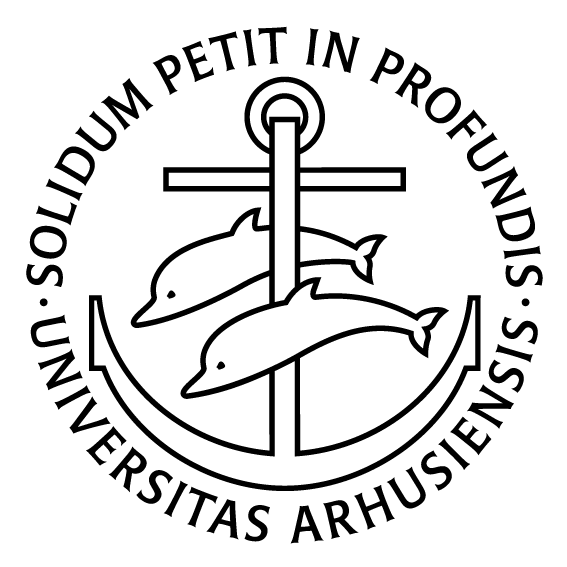
\includegraphics[width=0.5\textwidth]{ausegl_sort.png}
  \vspace{-10cm}
}

% \begin{centering}
  % 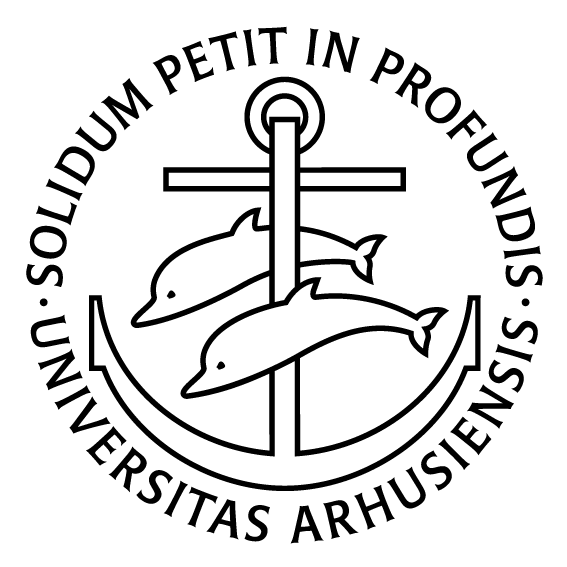
\includegraphics[width=0.5\textwidth]{ausegl_sort.png}
% \end{centering}
\vspace{0.5\textheight} % Whitespace between the title block and the publisher
\vfill
{\noindent Supervisor: Niels Lauritzen \hspace{2.5cm} 
\includegraphics{AU_logo.png}  }\\[\baselineskip] % Publisher and logo
}%}
% \endgroup
}

\begin{document}
% \maketitle
\titleGM
% \vfill
% Vejleder: Niels Lauritzen
% \strut\hfill
% 
\includegraphics[right]{AU_logo.png}
\newpage
\tableofcontents

\newpage

\section*{Introduction}


\section{Preliminaries}
This project will assume familiarity with ring theory, multivariate polynomials over fields. A familiarity with Gröbner bases will be beneficial, but we will introduce the necesary notations and definitions. Let $R$ be a Noetherian, commutative ring and $X = (x_{1}, x_{2}, \dots, x_{n})$ be an ordered collection of symbols. We denote the ring of polynomials in these variables $R[X]$. Given two (disjoint) sets of variables $X$ and $Y$, we will use $R[X, Y]$ to mean $R[X \cup Y]$, which is naturally isomorphic to $R[X][Y]$. A monomial is a product of variables and a term is a monomial times a coefficient. We denote a monomial as $X^{v}$ for some $v \in \N^{n}$.

\begin{definition}[Monomial order, leading term]
  A \textit{monomial order} is a total order $<$ on the set of monomials satisfying that $u < v \implies wu < wv$.

  Given a monomial order $<$ and a polynomial $f \in R[X]$, the \textit{leading term} of $f$ is the term with the largest monomial w.r.t. $<$ and is denoted by $\LT_{<}(f)$. If $\LT_{<}(f) = a\cdot m$ for some monomial $m$ and $a \in R$, then we denote $\LM_{<}(f) = m$ and $\LC_{<}(f) = a$. If $<$ is clear from context, it will be omitted.
\end{definition}

These definitions naturally extend to sets of polynomials, so given a set of polynomials $F \subset k[X]$, we denote $\LM_{<}(F) := \{\LM_{<}(f) \mid f \in F\}$. The above definitions work over a general ring (and we will use that), for from here, we'll work over a field $k$. With this, we can give the definition of a Gröbner basis.

\begin{definition}[Gröbner basis]
  Let $G \subset k[X]$ be a finite set of polynomials and $<$ be a monomial order. We say $G$ is a \textit{Gröbner basis} if
  $\langle \LT_{<}(G) \rangle = \LT_{<}(\langle G \rangle )$
\end{definition}

\section{Definitions and initial results}
The purpose of this project is to study parametric Gröbner bases, so let's introduce those. The bare concept is rather simple.

\begin{definition}[Parametric Gröbner basis]
  Let $k$, $k_{1}$ be fields, $U$ and $X$ be collections of variables and $F \subset k[U, X]$ be a finite set of polynomials. A \textit{parametric Gröbner basis} is a finite set of polynomials $G \subset k[U, X]$ such that $\sigma(G)$ is a Gröbner basis of $\langle \sigma(F) \rangle$ for any ring homomorphism $\sigma : k[U] \to k_{1}$.
\end{definition}

We call such a $\sigma : k[U] \to k_{1}$ a \textit{specialization}. By the linearity of $\sigma$, all such ring homomorphisms can be characterized by their image of $U$. Thus, we can identify $\{\sigma : k[U] \to k_{1} \mid \sigma \text{ is a ring hom.}\}$ with the affine space $k_{1}^{m}$ when $U$ has $m$ elements. For $\alpha \in k_{1}^{m}$ we'll denote the corresponding map
\[\sigma_{\alpha}(u_{i}) = \alpha_{i} \quad \text{for $u_{i} \in U$}\] extended linearly.

When we work with these parametric Gröbner bases, it will be more convenient to have a bit more information attached to them, namely which elements are required for which $\sigma$. Since $\sigma$ is described by an $\alpha \in k_{1}^{m}$, we can restrict them using subsets of $k_{1}^{m}$.

\begin{definition}[Vanishing sets \& algebraic sets]
  Let $E$ be a finite subset of $k[X]$. Then the \textit{vanishing set} of $E$ is $V(E) := \{v \in k^{n} \mid e(v) = 0 \;\; \forall e \in E\}$.

  An \textit{algebraic set} is a set of the form $V(E) \setminus V(N)$ for two finite subsets $E$ and $N$ of $k[X]$.
\end{definition}

\begin{definition}[Gröbner system]
  Let $A$ be an algebraic set and $G \subset k[U, X]$ be a finite set. Then $(A, G)$ is called a \textit{segment of a Gröbner system} if $\sigma_{\alpha}(G)$ is a Gröbner basis of $\sigma_{\alpha}(\langle G \rangle)$ for all $\alpha \in A$. A set $\{(A_{1}, G_{1}), \dots, (A_{t}, G_{t})\}$ is called a \textit{Gröbner system} if each $(A_{i}, G_{i})$ is a segment of a Gröbner system.
\end{definition}

\begin{example}
  Let $X = \{x, y\}$ and $U = \{u\}$ and consider the polynomials $f(x, y, u) = ux^{2} + x$ and $g(x, y, u) = xy + 1$. When $u \neq 0$, a Gröbner basis of $\langle f, g \rangle$ could be $(y-u, ux + 1)$, whatever $u$ may be. \colorbox{red}{TODO}
\end{example}

\colorbox{red}{Skriv om Kalkbrener}
\begin{definition}[Leading coefficient w.r.t. variables]
  Let $f \in k[U][X]$. Then the leading term of $f$ is denoted $\LT_{U}(f)$, the leading coefficient is $\LC_{U}(f)$ and the leading monomial is $\LM_{U}(f)$. These notations are also used when $f \in k[U, X]$, just viewing $f$ as a polynomial in $k[U][X]$.
\end{definition}

Note that $\LC_{U}(f) \in k[U]$, i.e. the leading term is a polynomial in $k[U]$ times a monomial in $X$.

From this point, we assume that the monomial order on $k[U, X]$ satisfies $x > u$ for all $x \in X$ and $u \in U$. This monomial order restricts to a monomial order on $k[X]$, denoted by $<_{X}$. Note that this assumption is not too restrictive, as both the lexicographic, reverse lexicographic and graded versions of those satisfies this assumption.

\begin{lemma}\label{lem:grb_iff_reduc_to_z}
  Let $G$ be a Gröbner basis of an ideal $\langle F \rangle$ w.r.t. $<$, let $\alpha \in k_{1}^{m}$ and set $G_{\alpha} := \{\sigma_{\alpha}(g) \in G \mid \sigma_{\alpha}(\LC_{U}(g)) \neq 0\} = \{g_{1}, g_{2}, \dots, g_{l}\} \subset k_{1}[X]$. Then $G_{\alpha}$ is a Gröbner basis of the ideal $\langle \sigma_{\alpha}(F) \rangle$ w.r.t. $<_{X}$ if and only if $\sigma_{\alpha}(g)$ is reducible to 0 modulo $G_{\alpha}$ for every $g \in G$.
\end{lemma}
\begin{proof}
  To we written after \colorbox{red}{Kalkbrener}
\end{proof}


We will use this lemma in a slightly different formulation:

% \begin{lemma}
%   Let $G = \{g_{1}, g_{2}, \dots, g_{k}\}$ be a Gröbner basis of an ideal $\langle F \rangle$ in $k[U, X]$ w.r.t $<$ and let $\alpha \in V(G \cap k[U])$. If $\sigma_{\alpha}(\LC_{U}(g)) \neq 0$ for each $g \in G \setminus (G \cap k[U])$, then $\sigma_{\alpha}(G)$ is a Gröbner basis of $\langle \sigma_{\alpha}(F) \rangle$.
% \end{lemma}
% \begin{proof}
%   Since $\alpha \in V(G \cap k[U])$ and $\LC_{U}(g) = g$ for any $g \in G \cap k[U]$, we have that $\sigma_{\alpha}(\LC_{U}(g)) = 0$ for all $g \in G \cap K[U]$. By assumption, $\sigma_{\alpha}(\LC_{U}(g)) \neq 0$ for any $g \notin G \cap k[U]$, thus $\sigma_{\alpha}(\LC_{U}(g)) = 0 \iff g \in G \cap k[U] \iff \sigma_{\alpha}(g) = 0$.

%   Now, $G_{\alpha} = \{\sigma_{\alpha}(g) \mid \sigma_{\alpha}(\LC_{U}(g)) \neq 0\}$ and take any $g \in G$. If $\sigma_{\alpha}(g) \in G_{\alpha}$, then $\LT(\sigma_{\alpha}(g)) = \sigma_{\alpha}(\LC_{U}(g)) \cdot \LM_{U}(g)$ since $x > u$ for all $x \in X$ and $u \in U$. Thus, $\sigma_{\alpha}(g)$ is reducible to $0$ modulo $G_{\alpha}$, since it's leading term is divisible by its own leading term.  On the other hand, if $\sigma_{\alpha}(g) \notin G_{\alpha}$, then $\sigma_{\alpha}(g) = 0$, so is immediately reducible to zero.
% \end{proof}


\begin{lemma}
  Let $G = \{g_{1}, g_{2}, \dots, g_{k}\}$ be a Gröbner basis of an ideal $\langle F \rangle$ in $k[U, X]$ w.r.t $<$ and let $\alpha \in k_{1}^{m}$. If $\sigma_{\alpha}(\LC_{U}(g)) \neq 0$ for each $g \in G \setminus (G \cap k[U])$, then $\sigma_{\alpha}(G)$ is a Gröbner basis of $\langle \sigma_{\alpha}(F) \rangle$.
\end{lemma}
\begin{proof}
  Let $G_{\alpha} = \{\sigma_{\alpha}(g) \mid \sigma_{\alpha}(\LC_{U}(g)) \neq 0\}$. If there is any $g \in G$, such that $\sigma_{\alpha}(g) \in k_{1} \setminus \{0\}$, then $g \in G \cap k[U]$ since $\sigma_{\alpha}(\LC_{U}(g)) \neq 0$ for all $g \in G \setminus K[U]$. Furthermore, since $g \in \langle F \rangle$, we get that $\langle \sigma_{\alpha}(F) \rangle = k_{1}[X]$ and $\sigma_{\alpha}(G)$ is a Gröbner basis.

  If there is no such $g$, then $\alpha \in V(G \cap k[U])$. Take any $g \in G$. If $\sigma_{\alpha}(g) \in G_{\alpha}$, then $\LT(\sigma_{\alpha}(g)) = \sigma_{\alpha}(\LC_{U}(g)) \cdot \LM_{U}(g)$ since $x > u$ for all $x \in X$ and $u \in U$. Thus, $\sigma_{\alpha}(g)$ is reducible to $0$ modulo $G_{\alpha}$, since it's leading term is divisible by its own leading term.  On the other hand, if $\sigma_{\alpha}(g) \notin G_{\alpha}$, then $\sigma_{\alpha}(g) = 0$, so is immediately reducible to zero. Thus $\sigma_{\alpha}(G)$ is a Gröbner basis of $\langle \sigma_{\alpha}(F) \rangle$ by lemma~\ref{lem:grb_iff_reduc_to_z}.
\end{proof}

With lemma~\ref{lem:grb_iff_reduc_to_z} in mind, we can start constructing Gröbner systems. Let $G$ be a reduced Gröbner basis of an ideal $\langle F \rangle \subset k[U, X]$, and let $H = \{\LC_{U}(g) \mid g \in G \setminus k[U]\}$. Then $\left(k_{1}^{m} \setminus \bigcup_{h \in H} V(h), G\right)$ is a segment of a Gröbner system. Thus, to make a Gröbner system, we need to find segments covering $\bigcup_{h \in H} V(h) = V(\lcm\{h \mid h \in H\})$.

If we take $G$ to be a reduced Gröbner basis, then $h \notin \langle F \rangle$ for any $h \in H$ since then the corresponding leading term would be divisible by a leading term in $G$. This is not allowed when $G$ is reduced. Hence, we can find a Gröbner basis $G_{1}$ of $F \cup \{h\}$, which will then form a segment $(k_{1}^{m} \setminus \bigcup_{h \in H_{1}} V(h), G_{1})$ where $H_{1} = \{\LC_{U}(g) \mid g \in G_{1}\}$. Since $k[U, X]$ is Noetherian, this will eventually stop, forming a Gröbner system.

This leads us to the first algorithm.







\printbibliography


\appendix


\end{document}
